\documentclass[12pt]{article}


\usepackage{amssymb}
\usepackage{amsmath}
\usepackage{fullpage}
\usepackage{epsfig}
\usepackage{epstopdf, hyperref, xcolor}
\everymath{\displaystyle}

\newif\ifans

\anstrue

\begin{document}

\begin{center}
\underline{\LARGE{Improper Integrals}}
\end{center}

\noindent SUGGESTED REFERENCE MATERIAL:

\bigskip

\noindent As you work through the problems listed below, you should reference Chapter 7.8 of the recommended textbook (or the equivalent chapter in your alternative textbook/online resource) and your lecture notes.

\bigskip

\noindent EXPECTED SKILLS:

\begin{itemize}

\item Given an improper integral, which either has an infinite interval of integration or an infinite discontinuity, be able to evaluate it using a limit. 

\item Know how to determine if such an integral converges (and if so, what it converges to) or diverges.

\end{itemize}

\noindent PRACTICE PROBLEMS:

\medskip

\noindent {\bf For problems 1-13, evaluate each improper integral or show that it diverges.}

\begin{enumerate}

\item $\int_{1}^{\infty}\frac{1}{\sqrt{x}}\,dx$ 

\ifans{\fbox{$\infty$}} \fi

\item $\int_{-\infty}^{3}\frac{3x}{x^2+1}\,dx$ 

\ifans{\fbox{$-\infty$}} \fi

\item $\int_{1}^{\infty}e^{-x}\,dx$ 

\ifans{\fbox{$\frac{1}{e}$}} \fi

\item $\int_{1}^{\infty}xe^{-3x^2}\,dx$ 

\ifans{\fbox{$\frac{1}{6}e^{-3}$}} \fi

\item $\int_{0}^{4}\frac{1}{x^{2/3}}\,dx$ 

\ifans{\fbox{$3\sqrt[3]{4}$}} \fi

\item $\int_{4}^{\infty}\frac{1}{(x-2)^3}\,dx$ 

\ifans{\fbox{$\frac{1}{8}$}} \fi

\item $\int_2^6 \frac{1}{\sqrt{x-2}} \,dx$

\ifans{\fbox{$4$}} \fi

\item $\int_0^2 \frac{2}{\sqrt{4-x^2}} \,dx$

\ifans{\fbox{$\pi$}} \fi

\item $\int_0^{\infty} \frac{1}{x^2+4x+5} \,dx$ (Hint: Complete the square)

\ifans{\fbox{$\frac{\pi}{2}-\tan^{-1}(2)$}} \fi

\item $\int_0^{\frac{\pi}{2}} \frac{\sin{x}}{\sqrt[3]{\cos{x}}} \,dx$

\ifans{\fbox{$\frac{3}{2}$}} \fi

\item $\int_{0}^{\frac{\pi}{2}} \sqrt{\tan{x}}\sec^2{x} \,dx$

\ifans{\fbox{$\infty$}} \fi

\item $\int_0^9 \frac{1}{\sqrt[3]{(x-1)^2}} \,dx$

\ifans{\fbox{9}} \fi

\item $\int_{0}^{1}\frac{1}{x\ln{x}}\,dx$ 

\ifans{\fbox{$-\infty$}} \fi

\item Find the value of the constant $k$ so that $\int_{-\infty}^{\infty} \frac{k}{1+x^2} \,dx=1$.

\ifans{\fbox{$\frac{1}{\pi}$}} \fi

\item Compute the exact area between the graph of $y=\frac{4}{x^2-1}$ and the $x$-axis for $x \geq 7$.

\ifans{\fbox{$2\ln{\left(\frac{4}{3}\right)}$}} \fi

\item Consider Gabriel's Horn (shown below) which is formed by revolving the curve $y=\frac{1}{x}$ on $[1,\infty)$ around the $x$-axis.

\begin{center}
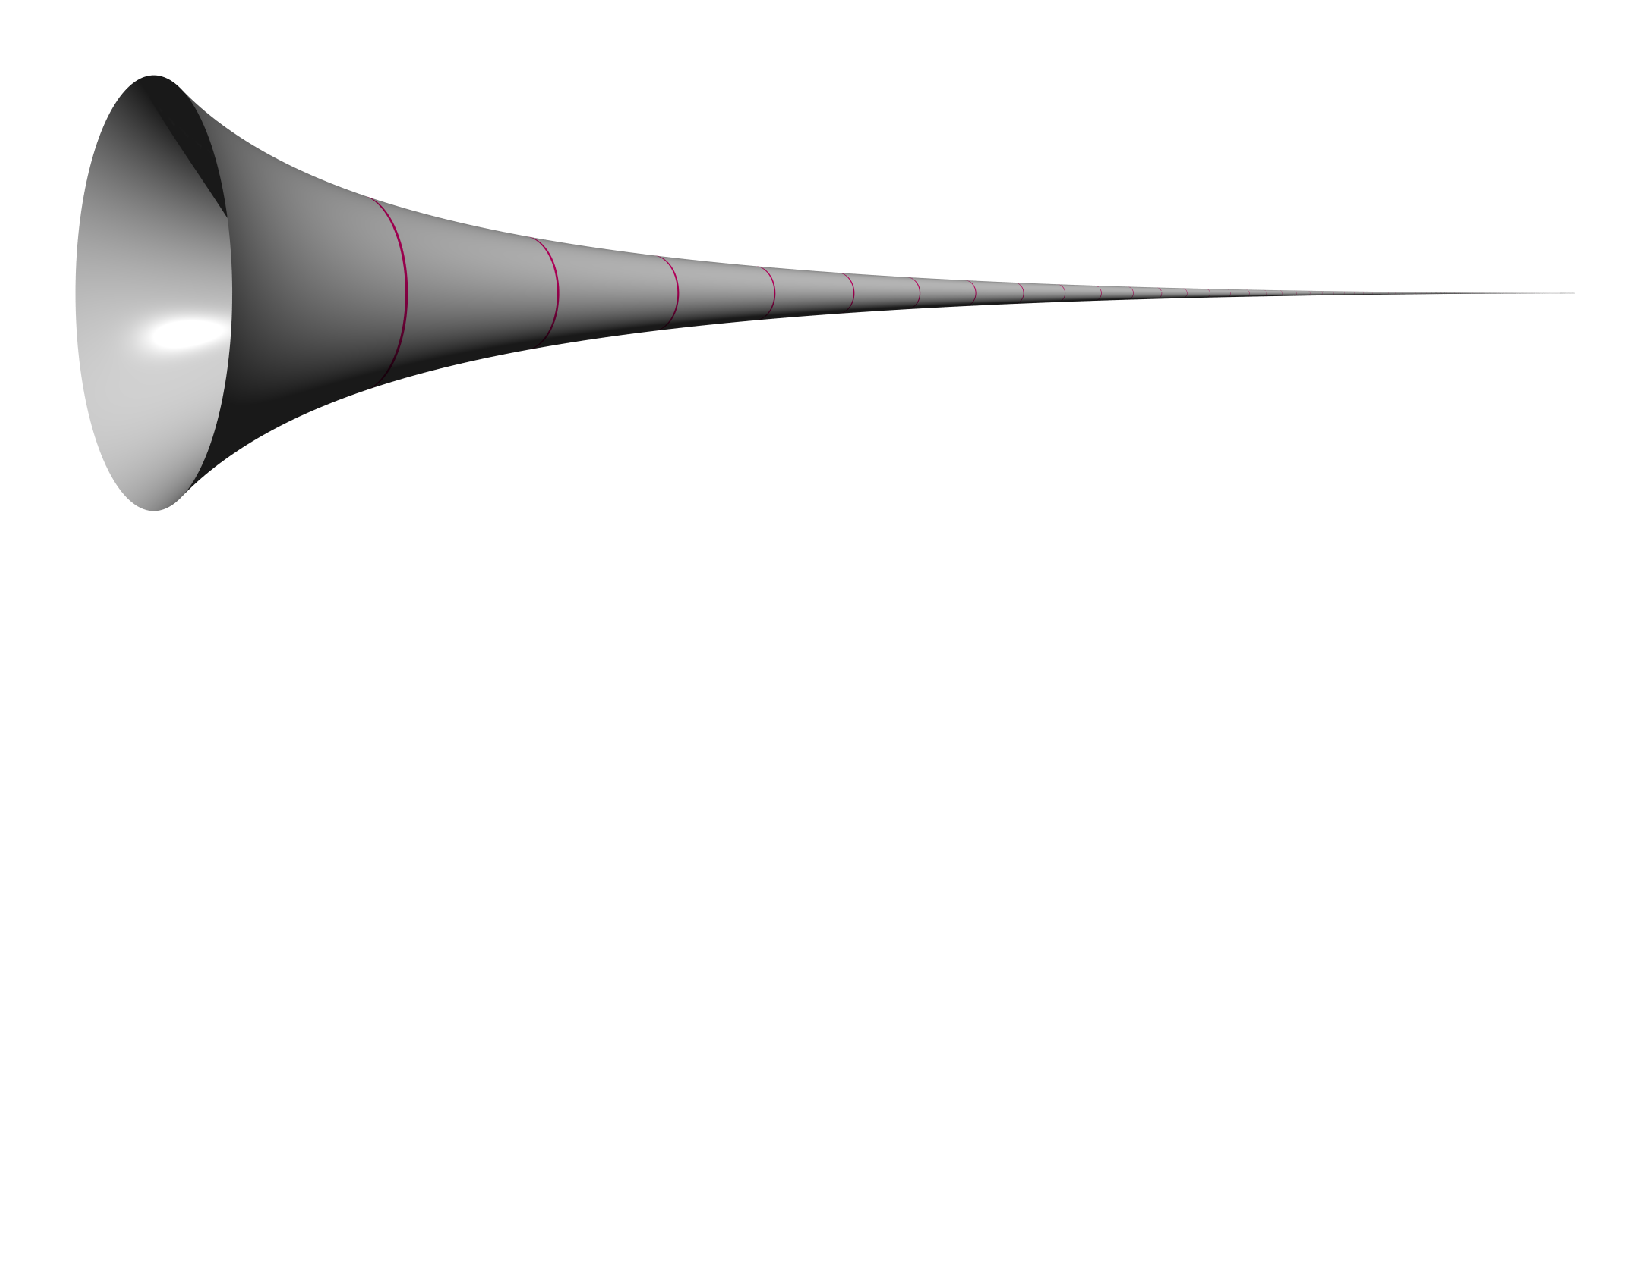
\includegraphics[scale=0.6]{GabrielHorn.pdf}
\end{center}

Show that the volume within this horn is finite.

\bigskip

Note: It can be shown the surface area of this horn is infinite.  Thus, it appears that the horn can be filled with a finite amount of paint; but, there is not enough to paint the inside of the surface for a coating of uniform thickness.  This is called {\bf The Paradox of Gabriel's Horn}.

\ifans{\fbox{$V=\pi$ cubic units}} \fi

\item Determine the values of the constant $p$ for which the following integral will converge and those for which it will diverge.  

$$\int_1^\infty \frac{1}{x^{^p}} \,dx$$

(Hint: Consider two cases -- when $p=1$ and when $p \neq 1$.)

\ifans{\fbox{Converges to $\frac{1}{p-1}$ if $p>1$; Diverges if $p \leq 1$; Detailed Solution: \textcolor{blue}{\href{http://www.math.drexel.edu/classes/Calculus/resources/Math122HW/Solutions/122_13_Improper_17.pdf}{Here}}}} \fi

\newpage

\item Determine the values of the constant $p$ for which the following integral will converge and those for which it will diverge.  

$$\int_0^1 \frac{1}{x^{^p}} \,dx$$

(Hint: Consider two cases -- when $p=1$ and when $p \neq 1$.)

\ifans{\fbox{Converges to $\frac{1}{1-p}$ if $p<1$; Diverges if $p \geq 1$}} \fi

\item Consider the Gamma Function: $\Gamma(\alpha)=\int_0^{\infty} x^{\alpha-1}e^{-x} \,dx$, which is defined for $\alpha>0$.

\begin{enumerate}

\item Compute $\Gamma(1)$.

\ifans{\fbox{1}} \fi

\item Compute $\Gamma(2)$.

\ifans{\fbox{$1$}} \fi

\item Compute $\Gamma(3)$.

\ifans{\fbox{$2$}} \fi

\end{enumerate}

\item If $f(x)$ is a continuous for $x \geq 0$, the {\bf Laplace Transform} of $f(x)$ is given by: $$\mathcal{L}\left\{f(x)\right\}(s)=\int_0^{\infty} f(x)e^{-sx}\,dx$$
and the domain of $\mathcal{L}\left\{f(x)\right\}(s)$ is the set consisting of all numbers $s$ for which the integral converges.  Laplace Transforms are useful for solving differential equations

\begin{enumerate}

\item Compute the Laplace Transform of $f(x)=1$ and state its domain.

\ifans{\fbox{$\mathcal{L}\left\{1\right\}(s)=\frac{1}{s}$ for $s >0$}} \fi

\item Compute the Laplace Transform of $f(x)=e^x$ and state its domain.

\ifans{\fbox{$\mathcal{L}\left\{e^x\right\}(s)=\frac{1}{1-s}$ for $s >1$}} \fi

\item Compute the Laplace Transform of $f(x)=x$ and state its domain.

\ifans{\fbox{$\mathcal{L}\left\{x\right\}(s)=\frac{1}{s^2}$ for $s >0$}} \fi

\end{enumerate}

\item {\bf Definition:} In probability theory, the {\bf probability density function (pdf)} of a random variable $X$ is a function $f(x)$ from which we can compute the probability that $X$ lies in the interval $[a,b]$ as follows: $$P(a\leq X \leq b)=\int_a^b f(x) \,dx$$  And, in order for $f(x)$ to be a valid pdf, it must satisfy the following:

\begin{itemize}

\item $f(x) \geq 0$ for all values of $x$

\item $\int_{-\infty}^{\infty} f(x) \,dx=1$

\end{itemize}

\begin{enumerate}

\item Verify that $f(x)=\left\{\begin{array}{ll}
2e^{-2x} & x \geq 0\\
0 & x <0
\end{array}\right.$ is a valid probability density function.

\ifans{\fbox{\parbox{1\linewidth}{Notice that $f(x) > 0$ for all $x\geq 0$ because $e^{-2x}>0$; and $f(x)=0$ for $x<0$.  Thus, $f(x) \geq 0$ for all $x$.  Also, $$\int_{-\infty}^{\infty}f(x) \,dx=\int_0^{\infty}2e^{-2x} \,dx =1$$  Thus, $f(x)$ is a valid pdf.}}} \fi

\item Using the density function in part $a$, compute $P(0 \leq X \leq 1)$.

\ifans{\fbox{$\int_0^{1}2e^{-2x} \,dx=1-\frac{1}{e^2}$}} \fi

\item {\bf Definition:} The {\bf cumulative distribution function (CDF)} for a continuous random variable $X$ is defined as: $$F(t)=P(X \leq t)=\int_{-\infty}^t f(x) \,dx$$  This CDF describes the accumulation of probability up to the real number $t$.  Compute the CDF for the random variable $X$ which has the density function from part a.

\ifans{\fbox{The CDF is $F(t)=\int_{-\infty}^{t}f(x) \,dx=\int_{0}^{t}2e^{-2x} \,dx=1-e^{-2t}$ for $t \geq 0$ and 0 for $t<0$.}} \fi

\end{enumerate}

\end{enumerate}

\end{document}